\documentclass{procDDs}
\usepackage{epstopdf}

                                                  % load packages only if necessary

\title{Theoretical and Experimental Study of Diffraction by a Thin Cone}

\author{\textbf{Belous A.A.}, Korolkov A.I., Shanin A.V.}% List of authors with the
{Faculty of Physics, Lomonosov Moscow State University, Russia}                 % same affiliation,
                                                  % lecturer given in bold
{artem.belous@gmail.com}                                   % e-mail of lecturer
%
%                                                 % it is important not to have
%                                                 % blank lines between the
%                                                 % \author and \coauthor
%
%\coauthor{Name I. Coauthor}                       % Co-author(s) with
%{Institute, University, Country}                  % another affiliation
%{coauthor@e.mail }                                               % use such line
                                                  % if e-mail none available

\begin {document}

\maketitle

\index{Belous, A.A.}                              % write this for each author
\index{Korolkov, A.I.}                              % to generate the index
\index{Shanin, A.V.}                             %

\begin{abstract}   
   A problem of diffraction of acoustical waves by a thin rigid cone is studied. A direct diffraction experiment is used to measure the diffracted field on the surface of a thin cone. The experiment is performed using MLS (Maximum Length Sequence) method. The cases of axial and non-axial incidence are studied. The wavelength is small compared to the cone length. Boundary integral equation method is used to describe the field theoretically in parabolic approximation. The integral equation is solved numerically by iterations. The results of the experiment are compared with the results of the calculation.
\end{abstract}

\section{Introduction}

   Diffraction by a thin cone  attracts considerable attention of researchers. Several different approaches exist to developing both asymptotics of the diffracted field and the diffracted field itself.  First, there is a traditional asymptotic approach based on ray representation \cite{Popov}. Second, there is an approach based on the parabolic equation method \cite{Andronov}. Third, there is an approach based on boundary integral equation method for the parabolic equation in Cartezian coordinates \cite{Shanin1}. Also, there is an approach based on the Smyshlyaev's formula \cite{Smychlyaev}, and another one based on Kontorovich-Lebedev  integral representation \cite{Lyalinov}. Still, authors know no works devoted to experimental study of this problem. In this work the authors are trying to fill this gap. 
   
   A direct diffraction experiment is used to measure the diffracted field on the cone surface. The experiment is performed using MLS technique \cite{Shanin}. The receiver is put on the surface of the cone. After that the cone is irradiated by a point source from different directions so that the receiver is enlightened or shadowed. Boundary integral equation method in parabolic approximation  \cite{Shanin_parabolic} is used to validate the results of the experiment.
   

\section{Experiment}

\subsection{Description}
A narrow (the vertex angle is $2\alpha = 5.5 ^{\circ}$) 1 meter long duralumin cone (see Fig.~\ref{cone}) is hanged in free space. A small (the size is around 0.01 meter) microphone is placed on the surface of the cone. The cone is irradiated by a small sound source (its size is around 0.01 meter) from different directions so the microphone can be shadowed or enlightened (see Fig.~\ref{exp_scheme}). A miniature Knowles RAB-32257 armature driver is used as a source and a well-calibrated no-name microphone is used as a receiver. 

\begin{figure}[t!]\centering
	\includegraphics[width=.5\textwidth]{cone.jpeg}
	\caption{Photo of the duralumin cone with the microphone on its surface.}\label{cone}
\end{figure}


To conduct the experiment, MLS method is used \cite{Shanin}. The cone is irradiated with a pseudo-random signal and then impulse response of the acoustical path is calculated through calculating correlation of the MLS signal with the output signal.

\begin{figure}[t!]\centering
	\includegraphics[width=.5\textwidth]{experiment.eps}
	\caption{Experiment scheme, view from above.}\label{exp_scheme}
\end{figure}

The input MLS signal is correlated with the measured signal and impulse response is calculated. A region of interest corresponding to diffraction by the cone is cropped from impulse response. After that a frequency image of the impulse response is calculated and compared to theory.


\section{Theoretical description}

\subsection{Problem statement}
Let us consider a stationary 3D problem and omit the time-dependence $\exp\{-i\omega t\}$.
The acoustical field satisfies Helmholtz equation everywhere outside the cone:
\begin{equation}\label{helm}                     
\Delta \tilde{p} + k^2 \tilde{p} = 0,                                         
\end{equation}
where $\Delta$ is the Laplace operator, $\tilde{p}$ is the acoustic pressure, $k$ is the wavenumber. 

Let us compare the acoustical impedance of duralumin of which the cone is made with that of air in order to choose the boundary conditions. For air, the acoustical impedance $Z_{air} = \rho \cdot c \approx 1.2 \left[\textrm{kg}/\textrm{m}^3\right] \cdot 343 \left[\textrm{m/sec}\right] = 413 \left[\textrm{N}\cdot \textrm{sec/m}^3\right]$. For duralumin, the impedance is $Z_{dural} = \rho \cdot c_{||} \approx 2800 \left[\textrm{kg/m}^3\right] \cdot 6400 \left[\textrm{m/sec}\right] \approx 18 \cdot 10^6 \left[\textrm{N}\cdot \textrm{sec/m}^3\right]$, where $c_{||}$ is the speed of longitudinal waves in duralumin. According to Fresnel formulas that the authors rely on in this work, the reflection coefficient on air/duralumin boundary is $R = (Z_{dural} - Z_{air})/(Z_{dural} + Z_{air}) = 1$ with the accuracy $10^{-5}$ which means that this boundary is almost a perfectly rigid one. This gives us the right to supplement (\ref{helm}) with Neumann boundary conditions on air/duralumin boundary:

\begin{equation}
\frac{\partial \tilde{p}}{\partial \vec{n}}=0,
\end{equation}
where $\vec{n}$ is the vector normal to the cone surface. 

The statement of this problem should be supplemented with radiation conditions. Radiation conditions in the limiting absorption form would demand that for $k$ having a small positive imaginary part the scattered field should decay as $r \rightarrow \infty$.
%\begin{equation}\label{rad_helm}                     
%\tilde{p} = O(\rho^{-1}), \quad \left(\frac{\partial u}{\partial \rho} - ik\right) \tilde{p} = o(\rho^{-1}) \quad \textrm{as} \quad \rho \rightarrow \infty,         \end{equation}
 Meixner's condition of absence of a source at the tip should also be satisfied. See, for example \cite{Smychlyaev}.
%\begin{equation}\label{meixner_helm}                     
%\tilde{p} = O(1), \quad \nabla \tilde{p} = o(\rho^{-1/2}) \quad \textrm{as} \quad \rho \rightarrow \infty.
%\end{equation}


The cone is very narrow (the vertex angle is much smaller than 1 radian) so most of the waves are supposed to be scattered under small angles. This means that parabolic approximation can be used to describe the diffraction processes \cite{Shanin_parabolic}. Following the standard procedure the field is represented in the following form (see Fig.~\ref{cone_pic}) :
\begin{equation}
\label{parab_field}                     
\tilde{p}(x,r,\varphi)=\exp\left\lbrace ikx \right\rbrace p(x,r,\varphi),                                         
\end{equation}
where $p$ is a slow function of $x$, compared to the exponential factor, $(x, r, \varphi)$ are cylindrical coordinates. Substituting (\ref{parab_field}) to (\ref{helm}) and neglecting the small terms, get the approximate equation for $p$:

\begin{equation}\label{parab_eqn}                     
\left( \frac{\partial}{\partial x} + \frac{1}{2ik} \Delta_\perp \right) p = 0,                                 
\end{equation}
where 
\begin{equation}
\Delta_\perp = \left(\frac{1}{r}\frac{\partial}{\partial r}r\frac{\partial}{\partial r}+\frac{1}{r^2}\frac{\partial^2}{\partial \varphi^2}\right).
\end{equation}
This is the parabolic equation of the diffraction theory.

\begin{figure}[t!]\centering
	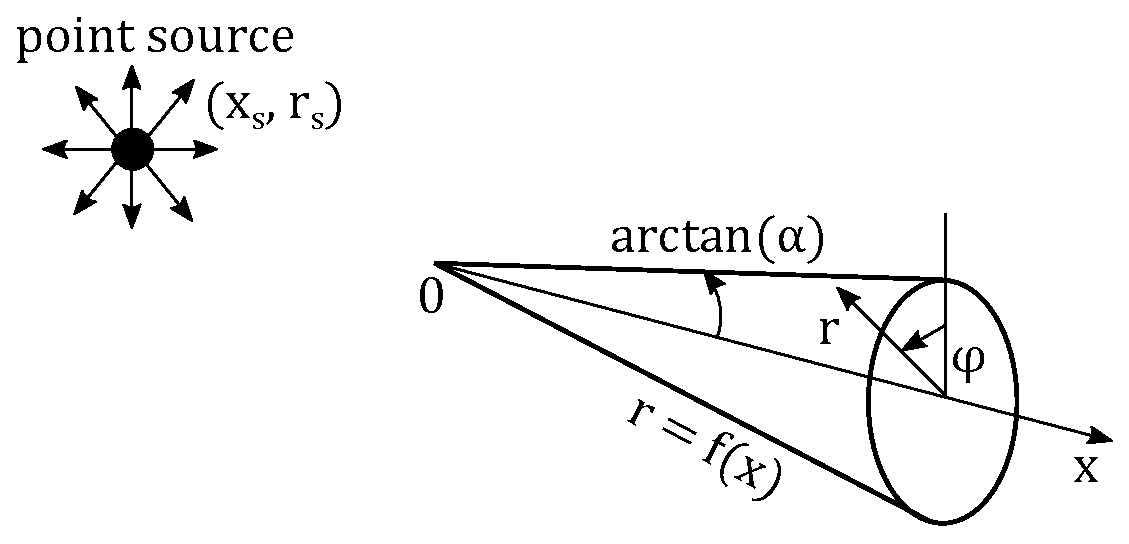
\includegraphics[width=.48\textwidth]{cone_pic.eps}
	\caption{Coordinate system of the experiment.}\label{cone_pic}
\end{figure}

The field $p$ is represented as a sum of the incident and the scattered field:
\begin{equation}
p = p^{\rm in} + p^{\rm sc}.
\end{equation}

As we are using a point source in the experiment, $p^{\rm in}$  is equal to Green's function of the parabolic equation. Let us denote the points of space by $\vec{r} = (x, r, \varphi)$ and the point source be located at $\vec{r_s} = (x_s, r_s, \varphi_s)$. Hence, 
\begin{equation}\label{greens_sol}                     
p^{\rm in} = \frac{k}{2\pi i (x-x_s)} \exp \left[   \frac{ik}{2} \frac{(\Delta r)^2}{x-x_s}\right], \quad x>x_s.
\end{equation}
where $\Delta r$ is the distance between the projections of $\vec{r}$ and $\vec{r_s}$ onto the transversal plane:
\begin{equation}\label{delta_r}                     
(\Delta r)^2 = r^2 + r_s^2 - 2r r_s \cos(\varphi - \varphi_s).
\end{equation}
Note that $p^{\rm in}$ is equal to zero if $x < x_s$ for both parabolic and Helmholtz formulations of the problem.

Unlike the Helmholtz equation, the parabolic equation describes only waves travelling in the positive direction. So there should be no scattered waves at $x < 0$. This means that the initial condition can be formulated:
\begin{equation}
p^{sc}(x, r, \varphi) = 0 \quad \textrm{for} \quad x < 0.
\end{equation}

Problem statement for the parabolic equation should also be supplemented with radiation conditions and Meixner's condition. The radiation conditions can be stated in a way similar to that for the Helmholtz problem, and the Meixner's condition should be slightly modified. The Meixner's condition for the parabolic formulation is as follows. An analog of energy-like combination for the Helmholtz equation 
\begin{equation}
|\nabla_\perp p|^2 + |p|^2
\end{equation}
should be integrable in any small domain of the space outside the cone. Here $\nabla_\perp$ is the gradient in the plane normal to the $x$-axis. For details, refer to \cite{Shanin_parabolic}.

\subsection{Calculating the diffracted field}

In this work, the authors directly apply the theoretical results derived in \cite{Shanin_parabolic} to the cone problem. In \cite{Shanin_parabolic}, a boundary integral equation is derived for the problem of diffraction by a body of revolution. In short, an equation for the total field is derived from Green's theorem for the parabolic equation. The derived equation can be applied to bodies having their radiuses dependent on $x$ like $r = f(x)$, where $f(x)$ is a linear function for the cone case.

Let $P(x,\varphi)$ be the total field on the surface, $P^{\rm in}$ be the incident field on the surface, i.e. 
\begin{equation}
P^{\rm in}(x,\varphi) \equiv p^{\rm in}(x,f(x),\varphi),
\end{equation}
\begin{equation}
P(x,\varphi) \equiv p(x,f(x),\varphi).
\end{equation}
 Denote $x_*, \varphi_*$ as the observation point coordinates on the cone surface. Then the following integral equation is satisfied:
\begin{multline}\label{int_eq} 
P(x_*, \varphi_*) = \int_{0}^{2\pi}\int_{0}^{x_*} K(x_*, \varphi_*, x, \varphi) P(x, \varphi) dx d\varphi \\
+ 2P^{\rm in}(x_*, \varphi_*),
\end{multline}
\begin{multline} \label{int_ker}                   
K(x_*, \varphi_*, x, \varphi) = \frac{ikf(x)}{2\pi} \times \\
\left[ \frac{\dot{f}(x)}{x_* - x} +\frac{f(x) - f(x_*) \cos(\varphi - \varphi_*)}{(x_* - x)^2}\right] \exp(\zeta),\\
\zeta =   \frac{ik}{2} \frac{f^2(x_*) + f^2(x) - 2f(x_*) f(x) \cos(\varphi - \varphi_*)}{x_* - x} ,
\end{multline}
For our case $f(x)$ is a linear function of $x$, $r = f(x) = x\tan\alpha  \approx x \alpha $, where $2\alpha$ is the angle at the vertex of our cone.

Note that equation (\ref{int_eq}) is of Volterra type with respect to variable $x$, and its kernel is of difference type with respect to variable $\varphi$.
This means that it can be solved using iterations with respect to $x$.

Let us solve the equation numerically using the method of approximation with linear basis functions \cite{Zenkevich}. The following basis functions $N_i(x)$ are used:
\begin{equation}
N_i(x) = 
\begin{cases}
& 0, x_{i-1}>x,\\
&(x-x_{i-1})/(x_{i} - x_{i-1}), x_{i}>x>x_{i-1},\\
&(x_{i+1}-x)/(x_{i+1} - x_i), x_{i+1}>x>x_i,\\
&0, x>x_{i+1},
\end{cases}
\end{equation}
i.~e. $N_i(x)$ is a triangle basis function.
The solution $P$ is sought in the form:
\begin{equation} \label{discr}
P(x, \varphi) \approx \sum_{i=1}^M P_i(\varphi) N_i(x),
\end{equation}
where $P_i(\varphi)$ are some unknown functions.
We substitute (\ref{discr}) to (\ref{int_eq}) and get the following system of linear integral equations:
\begin{multline} \label{final_eq}
P_i(\varphi_*)   = \sum_{j=1}^{M}\int_0^{2\pi}K_{ij}(\varphi_*,\varphi)P_j(\varphi)d\varphi + 2P^{\rm in}_i(\varphi_*), 
\\ i = 1...M,
\end{multline}
where
\begin{equation}
P^{\rm in}_i(\varphi_*) \equiv P^{\rm in}(x_i,\varphi_*),
\end{equation}
\begin{equation}
\label{K_mat}
K_{ij}(\varphi_*,\varphi) \equiv \int_0^{x_i}K(x_i,\varphi_*,x,\varphi)N_j(x)dx,
\end{equation}
One can notice that the integrand in (\ref{K_mat}) oscillates near the point $x=x_i$ which can possibly be a source of numerical errors. To solve this issue the contour of integration is slightly shifted to the upper complex half-plane where the kernel $K$ decays exponentially. 

Then, the system (\ref{final_eq}) is discretized  using finite difference method and solved with iterations for each wavenumber. 

%%\begin{figure}[t!]\centering
%%	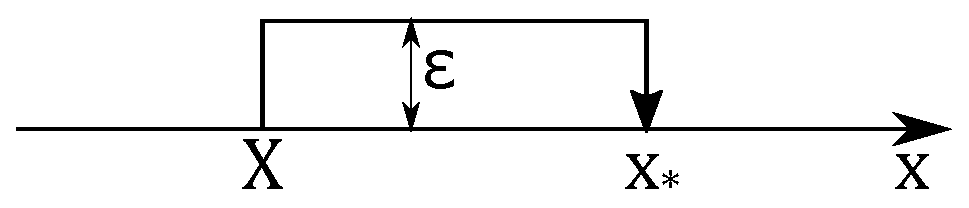
\includegraphics[width=.4\textwidth]{contour.eps}
%%	\caption{Integration contour for (\ref{contour}).}\label{contour}
%%\end{figure}
%
%Equation (\ref{final_eq}) can be solved by iterations with respect to $x$:
%
%\begin{align}                       % key is any name used
%& U(x) = \sum_{n=0}^{\infty} U^{\text{(n)}}(x) ,\notag\\
%& U^{(0)}(x) = 2U^{\text{in}}(x),\label{key3}\\
%& U^{(n+1)}(x_*) = \int_X^{x_*} K(x_*, x) U^{\text{(n)}}(x) dx, \quad n>0 \notag 
%\end{align}
%
%We calculate the solution for each frequency $\omega$ and finally we get $U(\omega)$ for the field in observation point (see Fig.~\ref{exp_scheme}). 


\section{Experimental results and modeling}

\subsection{Axial incidence}

In the case of axial incidence ($y_s = 0$) there was almost no diffraction observed, i. e. the field measured on the surface of the cone was close to the free field of the point source. This result may look a little surprising, but let us explain it in terms of Fresnel zone approach. It is supposed that diffraction on an obstacle occurs when the obstacle is covered by several Fresnel zones. Let us note that in our experiment we use the frequencies in range 2000 - 10000 Hz. In this range we can approximately suppose that the cone is irradiated by plane waves, since the source was 1 meter far from the cone's vertex. The difference of path lengths between the shortest ray and the ray diffracted by the cone can then be easily estimated (see Fig.~\ref{figFresnel}):
\begin{equation}
\label{Fresnel}
L_1 - L_0 = \Delta l(1 - \cos\alpha)\approx \Delta l \alpha^2/2,
\end{equation}
The first Fresnel zone size $\Delta l$ is determined by equating the latter to $\lambda/2$:     
\begin{equation}
\Delta l = \lambda/\alpha^2.
\end{equation}
Thus, for the highest frequency  the size of the first Fresnel zone $\Delta l$ is around 15 meters which is 15 times bigger than the total length of the cone. That is why we see no diffraction in the case of axial incidence. We should note that the same result is provided by the solution of equation (\ref{final_eq}). Also, a similar result for the case of elliptical cone is demonstrated in \cite{babich1995}.

%\begin{figure}[t!]\centering
%	\includegraphics[width=.5\textwidth]{axial.jpg}
%	\caption{Measured field for different $x$ for $f = 2000$ Hz (circles) and for $f = 3000$ Hz (stars) compared to geometrical fading $\sim 1/(x+1)$.}\label{axial}
%\end{figure}
\begin{figure}[t!]\centering
	\includegraphics[width=.5\textwidth]{Fresnel.eps}
	\caption{Illustration to calculation of the Fresnel zone size (\ref{Fresnel})}\label{figFresnel}
\end{figure}


\subsection{Non-axial incidence}
Using a calculation similar to (\ref{Fresnel}) one can show that diffraction process becomes more noticeable when the source is shifted towards the axis perpendicular to that of the cone. The experiment confirms this reasoning. The results of the experiment for shifts $y_s = \pm0.5, \pm0.3, \pm 0.1$ meters and $x_s =-1$ m  compared with the respective results of the solution of equation (\ref{final_eq}) is shown in Fig.~\ref{y01}, Fig.~\ref{y03}, Fig.~\ref{y05} correspondingly. The receiver was put near the surface of the cone with its $x$-coordinate equal to $0.8$ m, as shown in Fig.~\ref{exp_scheme}. We present the absolute values $|P/P_{\rm in}|$ to exclude the geometrical attenuation of the field. In other words, the value $P/P_{\rm in}$ can be considered as an approximation to the field of the plane wave diffraction problem.

\begin{figure}[t!]\centering
	\includegraphics[width=.5\textwidth]{y01.eps}
	\caption{Comparison of experiment and theory for $y = \pm 0.1$ m. Theory (solid line) and experiment (dashed line) for $y = -0.1$ m, theory (dotted line) and experiment (dash-dotted line) for $y = 0.1$ m.}\label{y01}
\end{figure}

\begin{figure}[t!]\centering
	\includegraphics[width=.5\textwidth]{y03.eps}
	\caption{Comparison of experiment and theory for $y = \pm 0.3$ m. Theory (solid line) and experiment (dashed line) for $y = -0.3$ m, theory (dotted line) and experiment (dash-dotted line) for $y = 0.3$ m.}\label{y03}
\end{figure}

\begin{figure}[t!]\centering
	\includegraphics[width=.5\textwidth]{y05.eps}
	\caption{Comparison of experiment and theory for $y = \pm 0.5$ m. Theory (solid line) and experiment (dashed line) for $y = -0.5$ m, theory (dotted line) and experiment (dash-dotted line) for $y = 0.5$ m.}\label{y05}
\end{figure}

The following natural conclusions can be made from the experiment. First, the absolute value of the field in the enlightened zone ($y_s < 0$) is bigger than in the shadow ($y_s > 0$). Second, the  value $|P/P_{\rm in}|$ in the enlightened zone tends to $2$ as frequency grows which corresponds to the case of reflection from hard wall, and tends to $0$ in shadow. 

The authors associate the theory-experiment discrepancies with positioning errors, electrical noises in the equipment, and imperfections of the source and microphone. Besides, for some wavenumbers the Neumann condition might fail due to interference of the surface waves excited in the cone with the incident spherical waves from the source. Also let us note that accuracy of the parabolic approximation decreases as $|y_s|$ grows, since the diffraction process cannot be considered paraxial. In the upcoming papers the authors are going to pay more attention to the problems mentioned and to provide comparisons with some other existing theoretical approaches \cite{Popov,Andronov,Smychlyaev,Lyalinov,babich1996}.     

%The experimental results highly depend on the phase shift which is technically the distance between the point source and the microphone. The distances in our experiments were measured with error about $\pm 1$ cm, so we attenuated the phase shift during the calculations by hand within $\Delta = 1$ cm via multiplying the field by $\exp(ik\Delta)$.



\section{Conclusion}

In this work, a direct  acoustical diffraction experiment has been held on diffraction by a narrow rigid cone with the use of a point source and MLS technique. The results of the experiment for axial incidence show that there is almost no diffraction due to a big longitudinal size of the Fresnel zone along the cone surface. For non-axial incidence (if the angle of incidence is small enough) the results agree with the solution of boundary integral equation in parabolic approximation.
 


%\iffalse 
%
%Body of subsection.
%
%Numbered formula should be written as
%\begin{equation}\label{key}                       % key is any name used
%a+b=2.                                         % to refer to the formula
%\end{equation}
%
%The reference to such an equation should be as (\ref{key}).
%
%A few formulae:
%\begin{gather}                       % key is any name used
%a+b=2,\label{key1}\\
%c+d=3.\label{key2}
%\end{gather}
%
%
%Aligned formulae:
%\begin{align}                       % key is any name used
%A={}&\int_0^1f(x)\mathrm{d}x,\notag\\
%&{}+a+b+c,\label{key3}\\
%B={}&3.\label{key4}
%\end{align}
%
%A long formula:
%\begin{multline}
%D=a+b+c+e+\sum_{n=1}^\infty t_n\\
%+f+\int_0^1g(x)\mathrm{d}x+q+h+y^2\\
%-r-s-\sin(w).
%\end{multline}
% 
%% See http://mirror.ctan.org/macros/latex/required/amslatex/math/amsldoc.pdf
%% for more examples of AMS-LaTeX commands.
% 
%Citations are written as \cite{paper1}.           % paper1 is the name from
%                                                  % \bibitem commands below
%Fig.~\ref{fig1} shows handling of figures.
%
%%\begin{figure}[t!]\centering
%%  \includegraphics[width=.43\textwidth]{Test_fig.eps}
%%  \caption{This is test figure}\label{fig1}
%%\end{figure}



\section*{Acknowledgements}

The work is supported by the RSF grant 14-22-00042.

%  citations should be arranged by order of appearance
%\fi
\begin {thebibliography}{9}
	
\bibitem{Popov} Popov A., Ladyzhensky A., Khozioski S., 2009, Uniform Asymptotics of the Wave Diffracted by a Cone of Arbitrary Cross Section,  \emph{Russ. J. Math. Phys.}. Vol. \textbf{16}, no. \textbf{2}, p. 296-–299.
	
\bibitem{Andronov} Andronov I. V., 2011, Diffraction by a Strongly Elongated Body of Revolution, \emph{Acoust. Phys.} . Vol. \textbf{57}, p. 147–-152.
	
\bibitem{Shanin1} A.\,V\;Shanin, A.\,I\;Korolkov, 2017,  Diffraction by a thin cone in the parabolic approximation. Method of the boundary integral equation, \emph{ICEAA Proceedings 2017}, DOI: 10.1109/ICEAA.2017.8065342
	
\bibitem{Smychlyaev} V.\,M\;Babich, D.\,B\;Dement'ev, B.\,A\; Samokish, V.\,P\; Smychlyaev, 2000, On evaluation of the diffraction coefficient for arbitrary "nonsingular" directions of a smooth convex cone, \emph{SIAM J. Appl. Math}, Vol. \textbf{60}, no. \textbf{2}, p. 536--573.
	
\bibitem{Lyalinov} Lyalinov M. A., Zhu N. Y., 2007, Acoustic scattering by a circular semitransparent conical surface, \emph{J. Eng. Math.}. Vol. \textbf{59}, no. \textbf{4}, p. 385--398.
	
\bibitem{Shanin} Shanin A. V., Valyaev V. Yu., 2011, Maximum length sequence method in diffraction experiment, \emph{Acoustical Physics}. Vol \textbf{57}, no. \textbf{3}, p. 420--425.

\bibitem{Shanin_parabolic} Shanin A. V., Korolkov A.I., 2018, Diffraction by an elongated body of revolution. A boundary integral equation based on the parabolic equation, \emph{arxiv.org} arXiv:1704.08857v1.

\bibitem{Zenkevich} Zienkiewicz~O.~C., Taylor~R.~L. The Finite element method Volume 1: The Basis,  Oxford, Butterworth-Heinemann, 2000.

\bibitem{Grikurov} Babich V. M., Lyalinov M. A., Grikurov V.E., Diffraction Theory. The Sommerfeld-Malyuzhinets Technique. \emph{Alpha Science International}, 2008.

\bibitem{babich1996} Babich V. M., 1996, The diffraction of a high-frequency acoustic wave by a narrow-angle absolutely rigid cone of arbitrary shape, \emph{J. Appl. Math. Mech.}, Vol. \textbf{60}, no. \textbf{1}, p. 72–-78.

\bibitem{babich1995} Babich V. M., Dement'ev D. B., Samokish B.A. 1995, On the diffraction of high-frquency waves by a cone of arbitrary shape, \emph{Wave Motion}, Vol. \textbf{21}, p. 203–-207.



\end{thebibliography}

\end {document}
